% $Id: template.tex 11 2007-04-03 22:25:53Z jpeltier $

\documentclass{vgtc}                          % final (conference style)
%\documentclass[review]{vgtc}                 % review
%\documentclass[widereview]{vgtc}             % wide-spaced review
%\documentclass[preprint]{vgtc}               % preprint
%\documentclass[electronic]{vgtc}             % electronic version

%% Uncomment one of the lines above depending on where your paper is
%% in the conference process. ``review'' and ``widereview'' are for review
%% submission, ``preprint'' is for pre-publication, and the final version
%% doesn't use a specific qualifier. Further, ``electronic'' includes
%% hyperreferences for more convenient online viewing.

%% Please use one of the ``review'' options in combination with the
%% assigned online id (see below) ONLY if your paper uses a double blind
%% review process. Some conferences, like IEEE Vis and InfoVis, have NOT
%% in the past.

%% Figures should be in CMYK or Grey scale format, otherwise, colour 
%% shifting may occur during the printing process.

%% These three lines bring in essential packages: ``mathptmx'' for Type 1 
%% typefaces, ``graphicx'' for inclusion of EPS figures. and ``times''
%% for proper handling of the times font family.

\usepackage{mathptmx}
%\usepackage{graphicx}
\usepackage[pdftex]{graphicx}
\usepackage{times}

%% We encourage the use of mathptmx for consistent usage of times font
%% throughout the proceedings. However, if you encounter conflicts
%% with other math-related packages, you may want to disable it.

%% If you are submitting a paper to a conference for review with a double
%% blind reviewing process, please replace the value ``0'' below with your
%% OnlineID. Otherwise, you may safely leave it at ``0''.
\onlineid{0}

%% declare the category of your paper, only shown in review mode
\vgtccategory{Research}

%% allow for this line if you want the electronic option to work properly
\vgtcinsertpkg

%% In preprint mode you may define your own headline.
%\preprinttext{To appear in an IEEE VGTC sponsored conference.}

%% Paper title.

\title{Solipsis: A Decentralized Architecture for Virtual Environments }

%% This is how authors are specified in the conference style

%% Author and Affiliation (single author).
%%\author{Roy G. Biv\thanks{e-mail: roy.g.biv@aol.com}}
%%\affiliation{\scriptsize Allied Widgets Research}

%% Author and Affiliation (multiple authors with single affiliations).
%%\author{Roy G. Biv\thanks{e-mail: roy.g.biv@aol.com} %
%%\and Ed Grimley\thanks{e-mail:ed.grimley@aol.com} %
%%\and Martha Stewart\thanks{e-mail:martha.stewart@marthastewart.com}}
%%\affiliation{\scriptsize Martha Stewart Enterprises \\ Microsoft Research}

%% Author and Affiliation (multiple authors with multiple affiliations)
\author{Davide Frey\thanks{e-mail:}\\ %
     \scriptsize Orange Labs%
\and Jerome Royan\thanks{e-mail: jerome.royan@orange-ftgroup.com}\\ %
        \scriptsize Orange Labs %
\and Romain Piegay \thanks{e-mail:romain.piegay@orange-ftgroup.com}\\ %
			\scriptsize Orange Labs \\%
\and Emmanuelle Anceaume \thanks{e-mail:}\\ %
			\scriptsize Orange Labs \\%
\and Anne-Marie Kermarrec \thanks{e-mail:}\\ %
			\scriptsize Orange Labs \\%			
}

%% A teaser figure can be included as follows, but is not recommended since
%% the space is now taken up by a full width abstract.
%\teaser{
  %\includegraphics[width=7in]{Teaser.pdf}
  %\caption{}
%}

%% Abstract section.
\abstract{
Lack of scalability is a key issue for virtual-environment technology, and more generally for any massive online experience because it prevents the emergence of a truly massive virtual-world infrastructure (Metaverse). The Solipsis project tackles this issue through the use of peer-to-peer technology, and makes it possible to build and manage a world-scale Metaverse in a truly distributed manner. Following a peer-to-peer scheme, entities collaborate to build up a common set of virtual worlds. We describe in this paper the communication protocol used to share data between peers connected together according to a N-Dimensional Voronoi based peer-to-peer network called RayNet. The policy of data exchange between peers takes advantage of the view-depedent representation used for 3D contents. Moreover, the solution proposed to distribute one each node processes usually executed on the server-side such as detection collision and physics computation. Finally, we present our web composant, a 3D navigator that can be easily executed on terminals with low ressources, and that provides solutions to swap between Web 2.0 and Web.

\textbf{Keywords:}
Peer-to-peer System, Metaverse, Shared Virtual Worlds, Massively Decentralized System, Adaptative 3D Streaming.

} % end of abstract

%% ACM Computing Classification System (CCS). 
%% See <http://www.acm.org/class/1998/> for details.
%% The ``\CCScat'' command takes four arguments.

\CCScatlist{ 
  \CCScat{K.6.1}{Management of Computing and Information Systems}%
{Project and People Management}{Life Cycle};
  \CCScat{K.7.m}{The Computing Profession}{Miscellaneous}{Ethics}
}

%% Copyright space is enabled by default as required by guidelines.
%% It is disabled by the 'review' option or via the following command:
% \nocopyrightspace

%%%%%%%%%%%%%%%%%%%%%%%%%%%%%%%%%%%%%%%%%%%%%%%%%%%%%%%%%%%%%%%%
%%%%%%%%%%%%%%%%%%%%%% START OF THE PAPER %%%%%%%%%%%%%%%%%%%%%%
%%%%%%%%%%%%%%%%%%%%%%%%%%%%%%%%%%%%%%%%%%%%%%%%%%%%%%%%%%%%%%%%%

\begin{document}

%% The ``\maketitle'' command must be the first command after the
%% ``\begin{document}'' command. It prepares and prints the title block.

%% the only exception to this rule is the \firstsection command
\firstsection{Introduction}

\maketitle

%\section{Introduction} 

The Metaverse concept, first described by Neal Stevenson in his
science fiction novel 'Snow Crash' published in 1992, and more
generally depicted in the whole cyberpunk writing movement, has deeply
influenced generations of virtual reality pioneers, artists, game
designers and nowadays virtual worlds enthusiasts. Over the last
sixteen years, the notion has evolved toward a synonym for virtual
world, loosing progressively the 'Universe' part of the concatenation
and the huge and infiniteness feeling emanating from it.

However, for us the Metaverse is a system of numerous, interconnected
virtual and typically user-generated worlds (or Metaworlds) all
accessible through a single-user interface. According to this strict
definition, the only Metaverse existing today is a prehistoric one:
the World Wide Web itself. Plenty of virtual worlds flourish these
days claiming they are the Metaverse, but they only are a part of it,
as websites are the leaves of the worldwide web tree. We need three
things to reach this cyberpunk authors' dream. First, a way to sustain
the incredible amount of data and MIPS involved, then a set of
protocols to provide interoperability and finally new tools to build
virtual worlds as easily as a traditional HTML page. These
requirements are the cornerstones of our project.

After a synthetic overview of the Solipsis research project (�I) and a
focus on related work (�II), we will describe how we envision to
manage decentralized virtual worlds, describing in details our
peer-to-peer architecture, and also how we manage 3D-model sharing and
physics computation. Finally, we will focus on how to stream 3D
contents in an adaptative\df{Where?????} way and then present our
navigator, which is the user interface used to interact with the Solipsis
Metaverse.


\section{Project overview}

In a word, Solipsis is a platform for massively multi-participant and
user-generated virtual worlds. It relies on a peer-to-peer
architecture that makes scalability its main characteristic: the
universe may thus be inhabited by an unlimited number of participants. As
there is no central authority, the virtual universe is by definition
public and the inhabitants' freedom, as well as the world builders and
developers' imagination, are boundless.

\subsection{Expected results}

We seek to spark off the emergence of an unbounded public virtual
universe that is designed, created, run, but also potentially hosted,
by people throughout the world. Freedom can be spotted as the main
characteristic of this opensourced system (license GNU/GPL v2+)
because the virtual universe does not belong to any organization; it
belongs to all the users.

The major deliverable is a new network communication protocol adapted
to the strong constraints of self-produced environments, to massively
multi-user applications and to virtual reality, which make the system
more scalable as the resources its uses are those provided by its
users.

We also work on creating an ergonomic and user-friendly interface to
allow non-professional agents to easily create 3D scenes and contents
(declarative or automatic modeling, tagging..). Nevertheless, we do
not want to mark a break with the actual flat 2D web; rather, we aim
to start a smooth transition towards an immersive Internet making the
most of both 2D and 3D. As we will see in part �V, our navigator can
be embedded in a regular webpage - in-web world - or map regular
webpages as an interactive texture on any 3D surface - in-world web.

The last major expected results are some deep analysis on the customs (virtual social life, game, education, services..) to give directions for future developments.

\section{Related Work}
\subsection{Centralized Virtual Worlds}
\subsection{Peer to Peer Architectures}
\subsection{Peer to Peer Architectures for Virtual Worlds}
\section{Architecture Overview}
\label{sec:overview}

\begin{figure}
\center
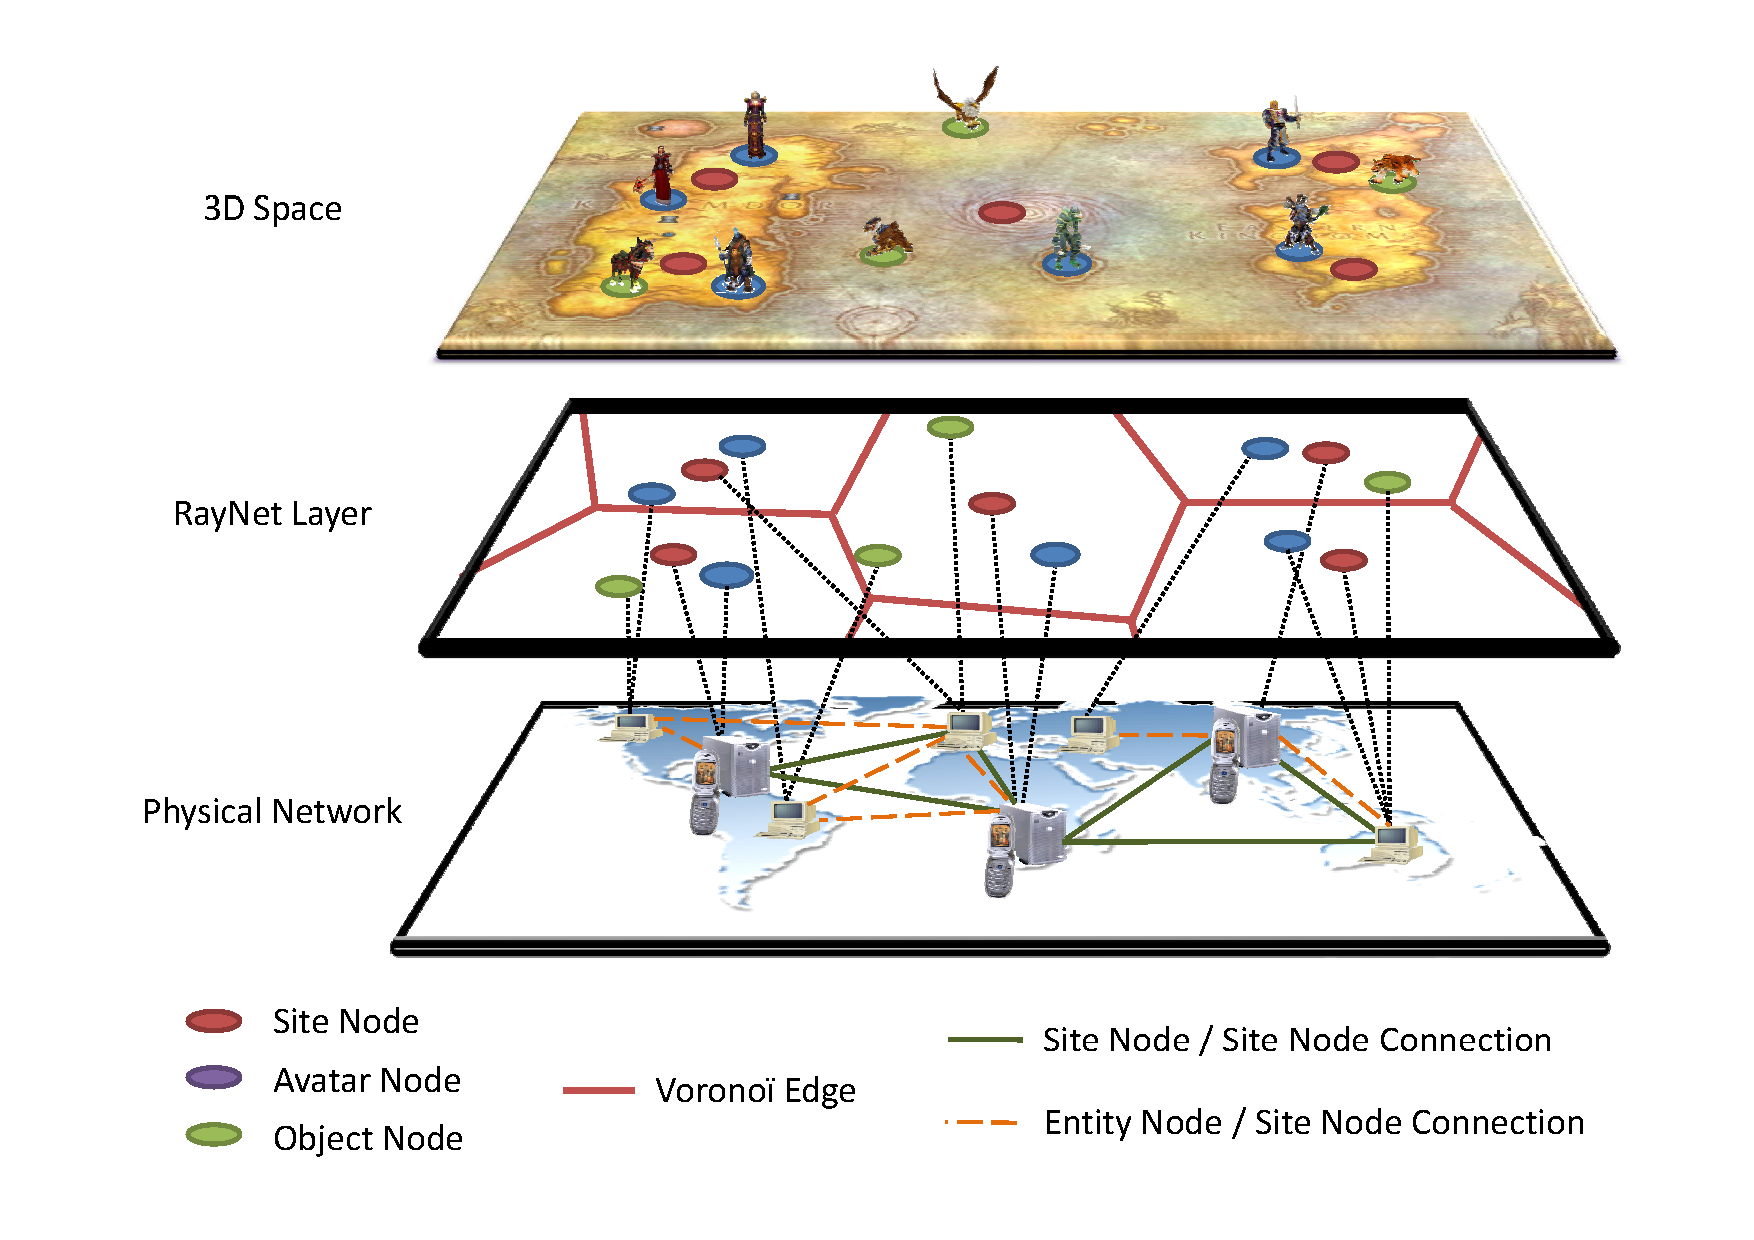
\includegraphics[width=3in]{Figures/Overview.pdf}
\caption{.}
\label{Fig:Overview}
\end{figure}

%figure showing the global architecture with vw layer, raynet layer, and host layer (text davide, figure jerome).
%figure showing Host + navigator (Jerome)


%%% Local Variables: 
%%% mode: latex
%%% TeX-master: MMVE
%%% End: 

\section{Decentralized Virtual Worlds Management}
\subsection{Definitions}
Objects, Sites, Avatars, descriptors.
\subsection{P2P Architecture}
RayNet, how does it work
\subsection{Decentralized 3D models sharing}
\subsection{Decentralized physics computation}
\section{3D streaming}
\subsection{context}
A user generated virtual environments is in perpetual evolution, requiring regular updates of the 3D models composing it. The actual solution consists in transmitting on the fly to the visualization client the different contents such as 3D models, images and videos. Streaming various media types, as opposed to the classical "download and play" paradigm, is already a widely used method, when the available bitrate is compatible with the quality required at rendering. 
In the case of 3D environments, the regions of interest are naturally the ones through which the user is roaming at a given time. As opposed to audio or video, the use of 3D content implies that the user is embedded within the media, and interacts with it. Hence, it is required that the environment be refined in real-time, according to the actual navigation and various interactions. The regions around the observer have naturally to be best refined, while the non-visible or distant regions can only be transmitted in coarser versions, ready to be refined when they become regions of interest.

\subsection{Adaptive 3D streaming}
In order to implement this so-called "view-dependency", several solutions can be considered. First, space partitionning is already a widely used method to filter the required contents according to the current viewpoint. The virtual environments are usually partitionned in cells thanks to a regular grid. When an avatar navigate into a cell, the server, or in our case peers, sent to the visualization client the contents present in this one. To reduce the amount of data to transmit over the network, 3D objects are generally represented using non-continuous level of details. Thus, a well-detailed representation of 3D contents close to the view point are sent to the client. Finally, a pre-loading of nearby cells can be done for anticipation.\\
This filtering solution, thanks to which visualized contents are progressively transmitted to visualization nodes according to their viewpoints, could be considered as an answer to adaptive streaming requirements. Moreover, the mapping of the Raynet layer into the virtual world provide us directly a space partitionning. But non-continuous level of details have the drawback to contain redundant information (as a level of detail does not use information from a lower level), and generally bring about popping effects when a model swap from one level of detail to the next one. For these reasons, the Solipsis framework supports continuous level of detail representations for textures, 3D models and animation.
\subsection{On-Demand 3D Streaming }
Autonomy of peers is a essential requirement to obtain a full scalable architecture. As explain previously, actual centralized architectures for virtual environments execute a significant amount of computation on the server-side.  Generally, clients have not a global knowledge of the scene, unlike servers that are mostly connected to a database containing a complete description of the 3D world. For these reasons, most of process such as level of detail selection,  collision detection, physics computation and animation are performed on the server side. Unfortunately, servers becomes quickly overloaded as the number of connected client increases. Only, as shown in \cite{Cavagna}, the complete model of the world is not necessary to compute the level of detail selection (the case of collision detections will be discussed in \ref{collision detection}). For 3D contents, Cavagna et al. disjoined the information required for rendering (3D model, textures, etc) to data used to select level of details. Thus, descriptors introduced in \ref{} are extended to include selection informations.     

   

\section{The navigator}
\label{sec:navigator}
A navigator must comply with some requirements to create a huge metaverse and democratize its use. First of all, the Ogre 3D rendering engine have been choosed for its robustness, efficiency, upgradability and openess that are necessary for a durable system. Moreover, Ogre 3D can be easily embedded in web pages thanks to a mozilla plugin or a ActiveX. Conversely, web pages can be mapped on 3D models as interactive textures thanks to the Navi library based on Gecko. Thus, the navigator allows a Web 2.0 navigation inside the Web 3D, as well as a Web 3D navigation inside the Web 2.0, as we clearly think that web 3D and web 2.0 are additional (see figure \ref{Fig:navigator}). 
\begin{figure}
\center
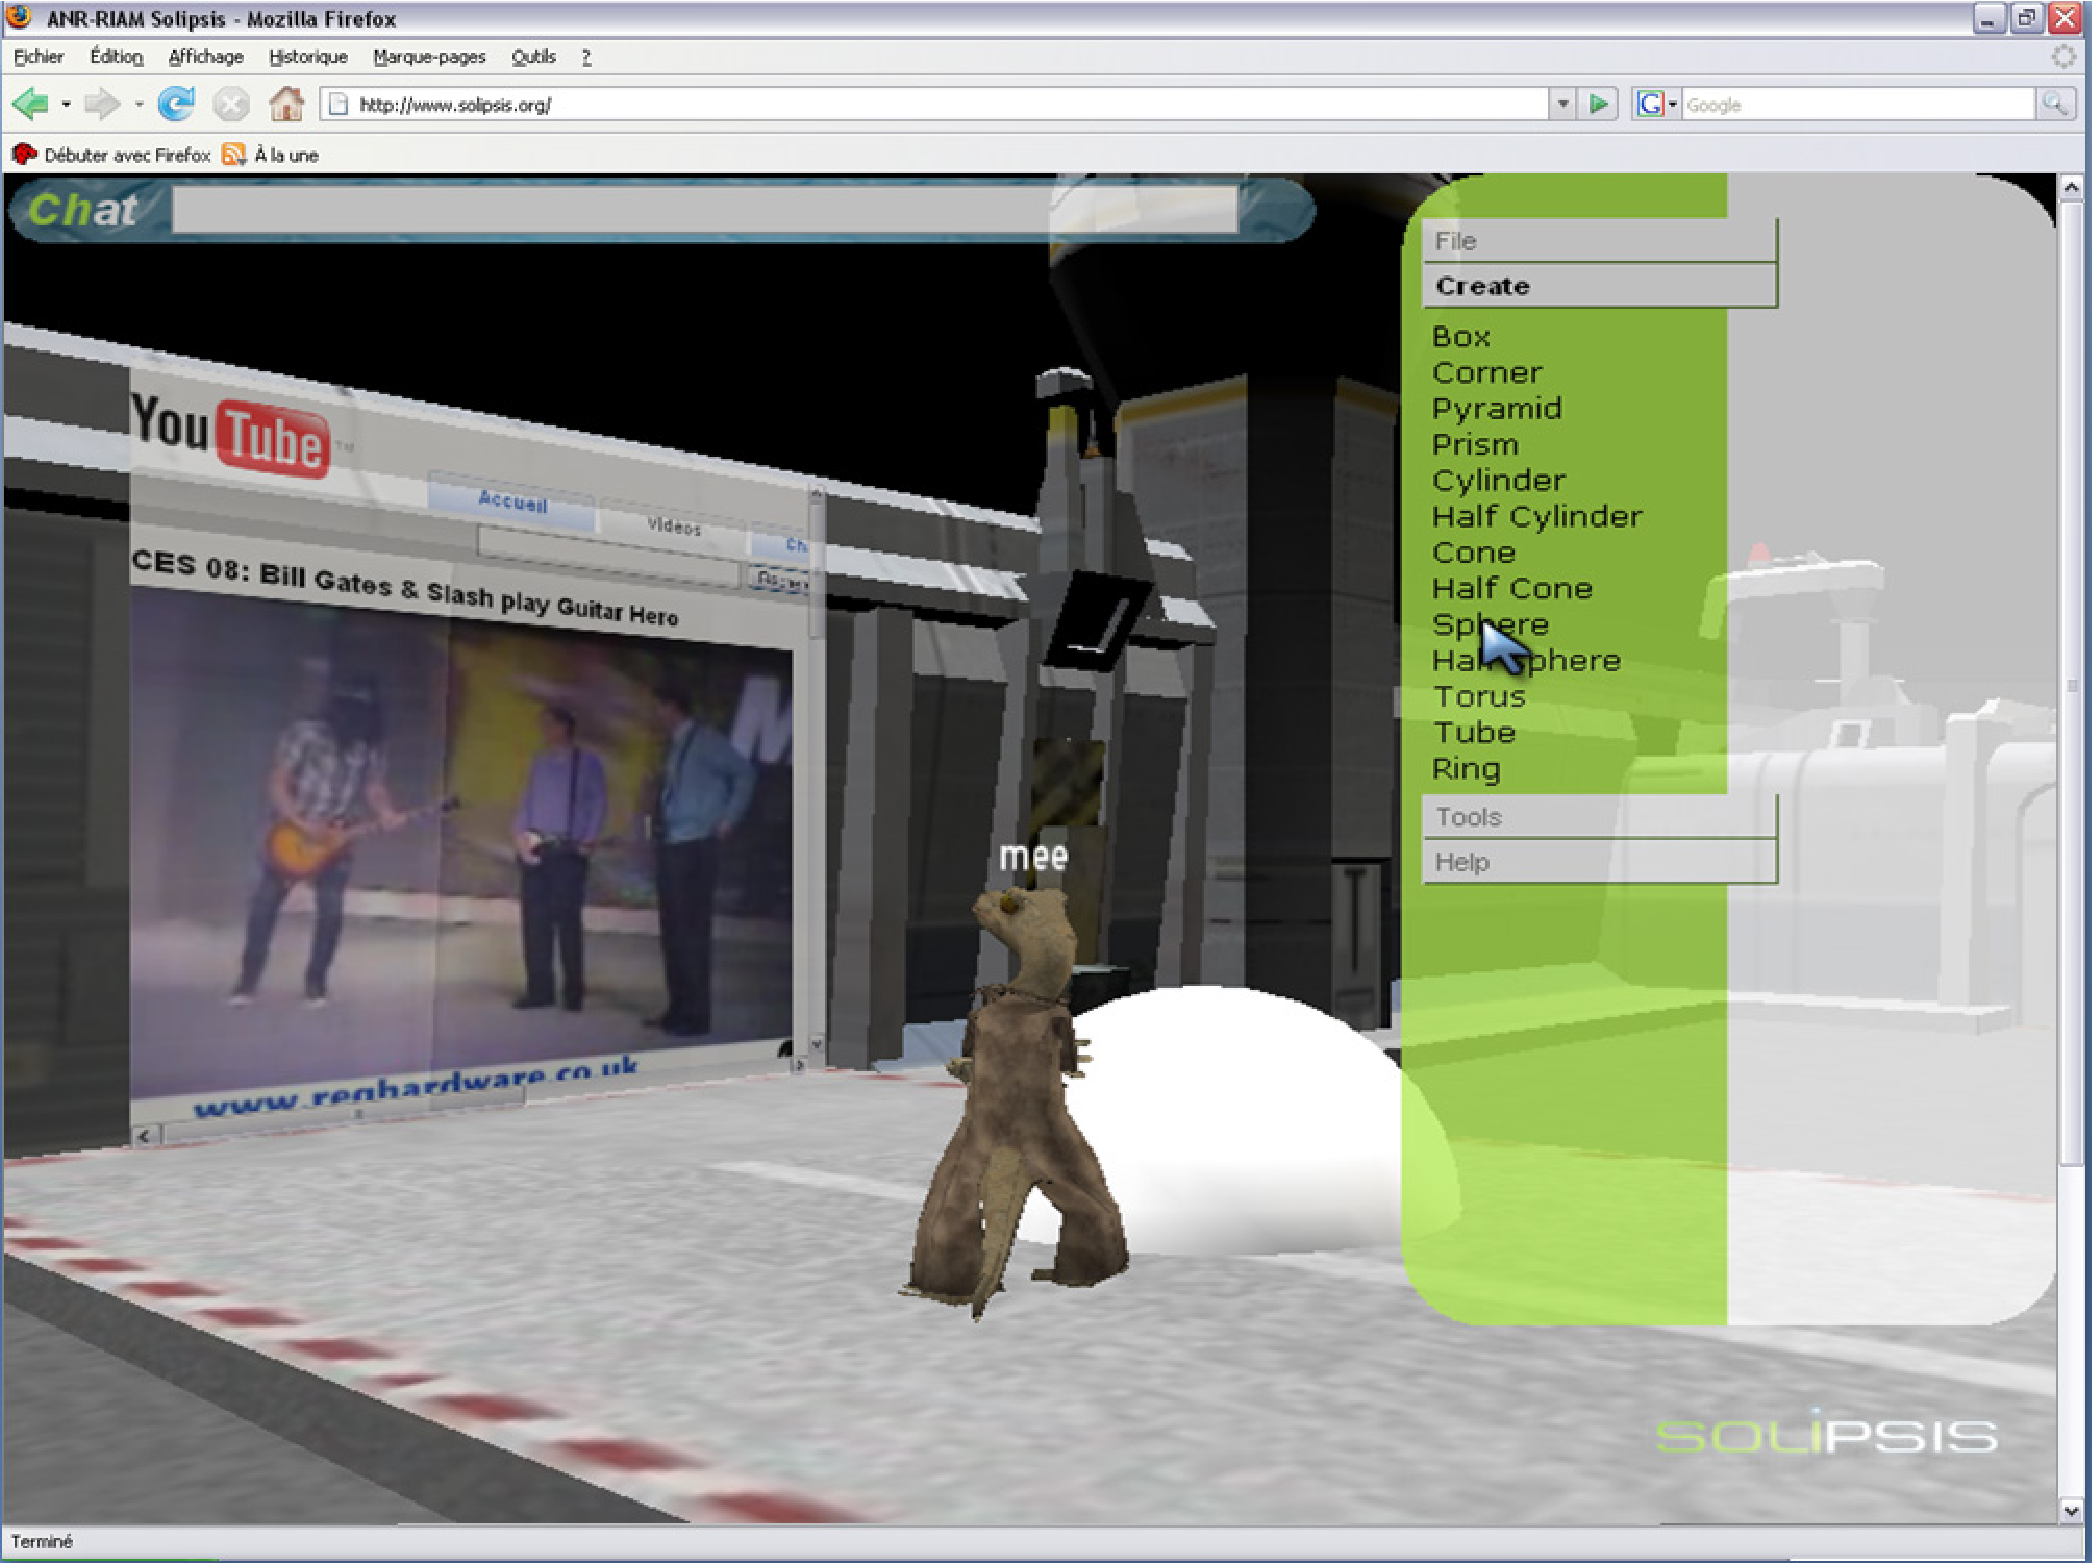
\includegraphics[width=3in]{Figures/navigator.pdf}
\caption{Web based navigator embedding modeling tools, and providing a mapping of web pages as interactive textures.}
\label{Fig:navigator}
\end{figure}
Since the vitual universe belongs to all users, modeling tools are embedded within the navigator in order to create, modify or delete contents. At the moment, we focus on intuitive tools, but procedural, declartive, parametric and sketching based modeling tools are obviously considered. Finally, to provide accesses to the virtual universe in mobility, nodes can be hosted by proxy servers, to reduce the amount of processes that have to be executed on terminals with low ressources. Thus, hosts can compute detection collision, physic animation, data exchange management, viewpoint based filtering, and communicate with the navigator that has just to render the virtual environment and interact with it (see figure \ref{Fig:host}).
\begin{figure}
\center
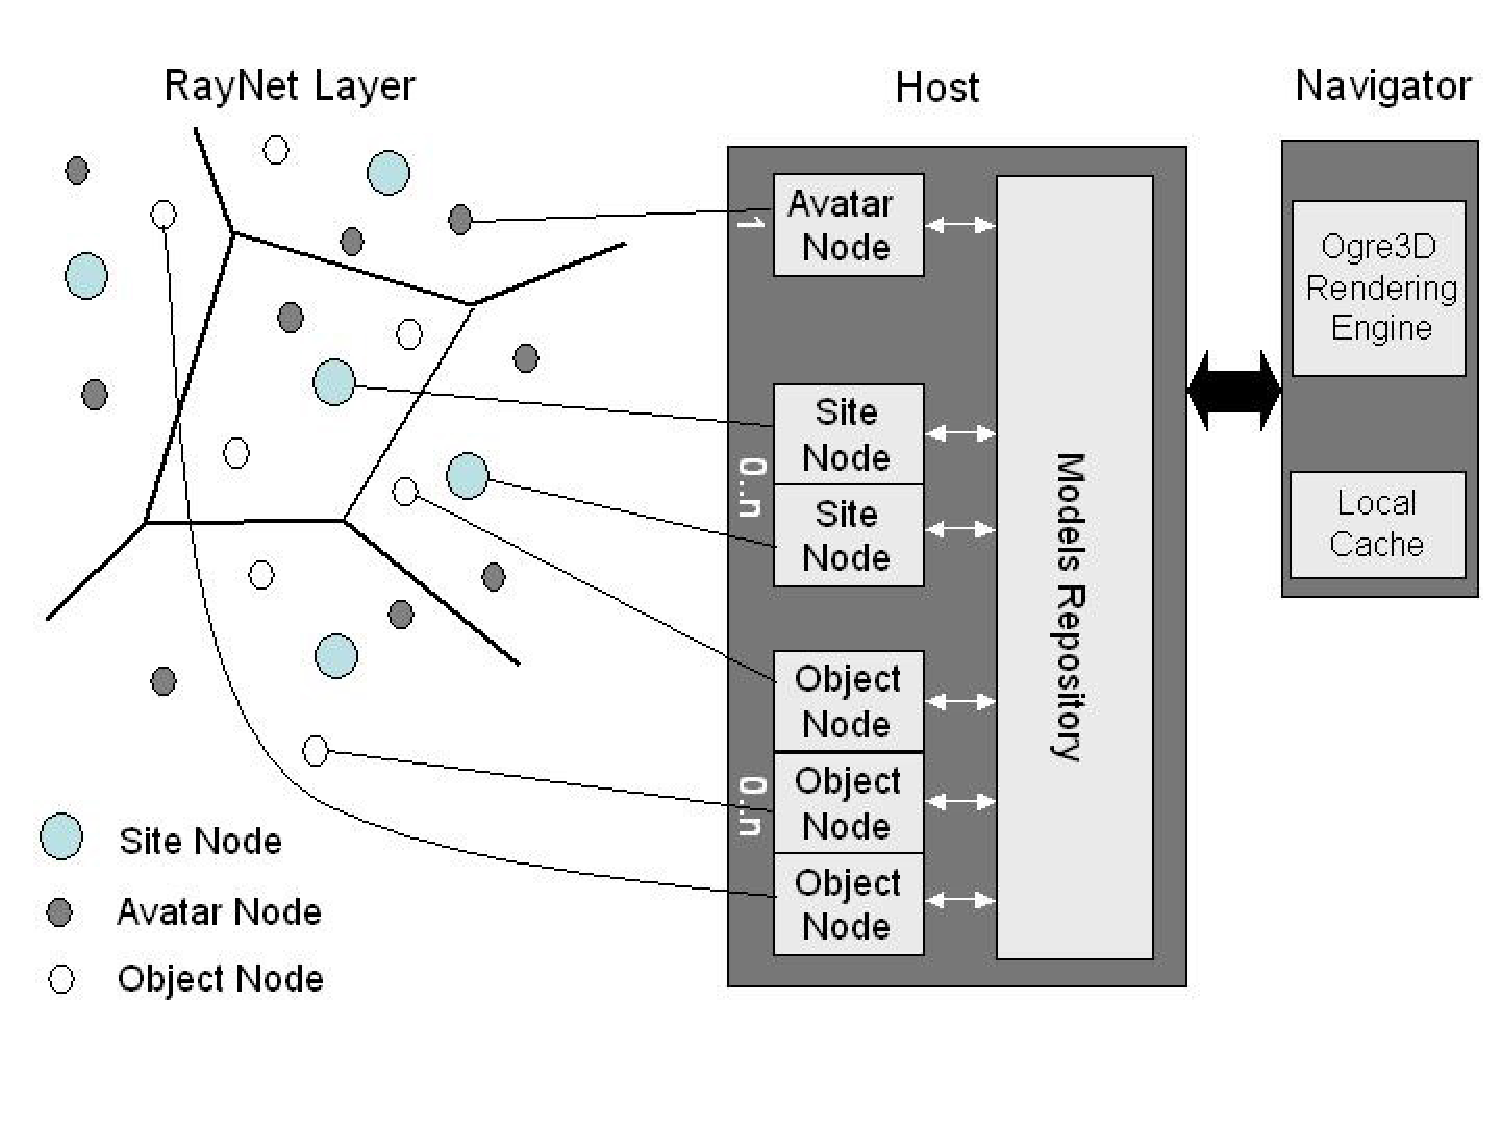
\includegraphics[width=3in]{Figures/host.pdf}
\caption{Nodes hosted on a proxy server to allow accesses to the metaverse on terminals with low ressources such as mobiles.}
\label{Fig:host}
\end{figure}
\section{Conclusions and perspectives}
We have presentd our vision of a decentralized architecture for virtual environments. Thanks to a N-dimensional Vorono� based p2p network, called RayNet, we can distibute the exchange of data and the computation of heavy tasks over the different nodes present in the virtual space. Descriptors presented in this papers allows us first managing with respect to view-dependency criteria the adaptive streaming of 3D models from neighborhood peers with the optimal resolution, and secondly filtering the computation of tasks such as detection collision according to the proximity between peers. Moreover, we have presented a management policy for objects to be able to use them, to control them using a user-defined software components, or to drop them in the virtual space. Finally, we describe the functionnalities of our navigator, allowing the visualization of Web 2.0 components into the virtual world , the embedding of the navigator into web pages thanks to interactive texuring, the modeling of 3D contents integrated to the viewer, and the possibility to interact with the universe from clients with low ressources such as mobile phones.\\
The use of a N-Dimensional p2p network allow us to extend the connectivity not only according to the proximity of peers in the virtual environment, but according to social or semantic proximity between object or avatar nodes. As the metaverse belong to all users, this project is fully opensource, and we hope that community will help us to improve our architecture and evaluate in full-size its effectiveness.  
       
%% if specified like this the section will be ommitted in review mode
\acknowledgements{
The authors wish to thank A, B, C. This work was supported in part by
a grant from XYZ.}

\bibliographystyle{abbrv}
%%use following if all content of bibtex file should be shown
%\nocite{*}
\bibliography{MMVE}
\end{document}
